\documentclass[12pt,a4paper]{article}
\usepackage[latin1]{inputenc}
\usepackage[spanish]{babel}
\usepackage{graphicx}
\usepackage[left=1.3cm,right=1.3cm,top=1.8cm,bottom=4cm]{geometry}
\usepackage{lastpage}
\usepackage{marginnote}
\usepackage{multirow}
\usepackage{wallpaper}
\usepackage{fancyhdr}
\setlength{\headheight}{87pt} 
\pagestyle{fancy}\fancyhf{}
\renewcommand{\headrulewidth}{0pt} 
\setlength{\parindent}{0cm}
\newcommand{\tab}{\hspace*{2em}}
\newcommand\BackgroundStructure{
	\setlength{\unitlength}{1mm}
	\setlength\fboxsep{0mm}
	\setlength\fboxrule{0.5mm}
	\put(10, 10){\fcolorbox{black}{white!10}{\framebox(192,247){}}}
	\put(10, 262){\fcolorbox{black}{white!10}{\framebox(192, 31){}}}
}

%-------------------------ENCABEZADO---------------
\fancyhead[L]{\begin{tabular}{l r | l r}	
		\textbf{Proyecto} & 1 & \textbf{Página} & \thepage/\pageref{LastPage} \\
		\textbf{Trabajo} & Desarrollo de un controlador & \textbf{Actualizado en:} & 27/08/2016 \\
		\textbf{} &  VGA & \textbf{Revisado en:} & 30/08/2016 \\
		\textbf{Grupo} & 1 & \textbf{Diseñadores} & Keylor Mena Venegas \\
		\textbf{Revisado por:} & Alfonso Chacón Rodríguez & \textbf{ } & Luis Leon Vega \\
		\textbf{} & & \textbf{ } & Luis Merayo Gatica
	\end{tabular}}

\begin{document}
\AddToShipoutPicture{\BackgroundStructure}

\section*{\textit{resumen}}
 
Se debe realizar un controlador para realizar la lectura y escritura del módulo RTC V3023. Los datos del sistema deben poder ser desplegados en un monitor LCD mediante el protocolo VGA. Ante ello, se debe realizar un controlador para el RTC y para la VGA. Asimismo, se deben poder ajustar la hora, activar la alarma y el cronómetro de forma descendente mediante botones e interruptores dispuestos en la FPGA Nexys3.\\

\section*{\textit{Introduccion}} 
Este proyecto consiste en realizar un controlador de módulos RTC (Real Time Controller), específicamente para el módulo V3023. Este controlador será capaz de escribir y leer dicho módulo para obtener parámetros de reloj, cronómetro y alarma. \\
Asimismo, para poder desplegar la información relevante de los parámetros anteriores, se conectará un monitor LCD mediante el protocolo VGA. Por otro lado, para poder programar y dar instrucciones al circuito, se deberán usar los botones señalados en el instructivo y algunos interruptores. \\
Finalmente, el conjunto es un circuito que permita controlar el módulo y comunicar al usuario mediante los botones y el monitor LCD, donde él podrá recibir la información relevante y poder modificar dicha información.\\

\section{Objetivos}
\begin{itemize}
	\item Diseñar un controlador de RTC que permita leerlo y programarlo mediante una interfaz de usuario consistente en botones incorporados dentro de la FPGA (Nexys3) y un monitor comunicado a través del protocolo VGA.
	\item Investigar el funcionamiento del módulo RTC y el protocolo de comunicación del mismo.
	\item Diseñar un controlador para el módulo RTC, cuyo bus de datos y direcciones estén multiplexados.
	\item Cumplir con las reglas de temporizado del sistema, en especial, con el protocolo de comunicación del módulo RTC.
	\item Combinar el controlador de RTC con un controlador VGA para poder desplegar la información del módulo al usuario. Este módulo VGA será adaptado del proyecto anterior.
	\item Desarrollar un banco de pruebas (testbench) para poder emular el comportamiento del módulo RTC con la finalidad de comprobar el funcionamiento del circuito controlador.
\end{itemize}

\section{Descripción del sistema}
El sistema se puede dividir en cuatro subsistemas, para facilitar el diseño dividimos el sistema en 4 grandes partes, el controlador de la pantalla, el controlador para el RTC, el control de usuario y  una memoria principal. Éstos subsistemas, pueden ser desarrollados de manera separada siempre que se tenga el cuidado necesario con los datos que comparten entre los bloques, para este efecto se desarrollo una memoria con 2 registros que se actualizan entre ellos al activar banderas. En la Fig. \ref{fig:sistema} se puede observar la composición general del sistema.

\begin{figure}[hbtp]
	\centering
	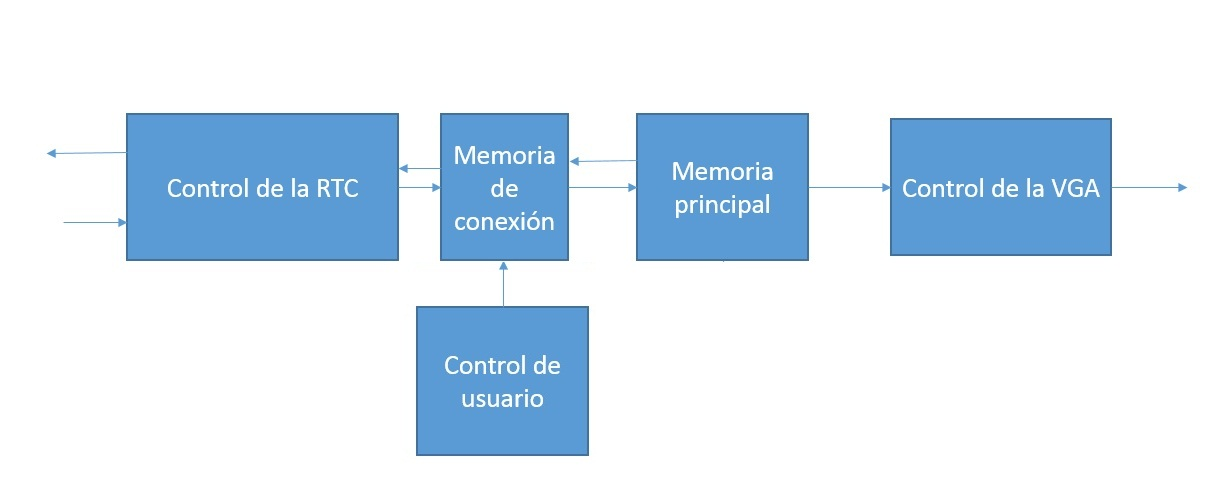
\includegraphics[height=8.5cm, width=18cm]{img/Subsistemas.jpg}
	\caption{Diagrama de modulos principales del sistema.}
	\label{fig:sistema}
\end{figure}

\subsection{Controlador de la pantalla}
\subsubsection{Diagrama de primer nivel}  \label{sec:VGA_pn}


\subsubsection{Diagrama de segundo nivel} \label{sec:VGA_sn}


\subsubsection{Diagrama de tercer nivel}


\subsection{Control de usuario}
Para poder controlar el acceso del usuario, que se comunica por medio de 7 botones, 3 interruptores que indican que se quiere cambiar, el reloj, el timer o la alarma, y para moverse entre los registros de datos y aumentar o disminuir sus valores.\\ 

\subsubsection{Diagrama de primer nivel}
el control de usuario posee 3 interruptores y 4 botones para que el usuario elija los datos y que desea cambiar. Ademas posee entradas y salidas de memoria para poder alterar los registros y escribirlos en la rtc. Se puede notar esto en la figura \ref{fig:PrimerNivelcontrolusr}.

\begin{figure}[htbp]
  \centering
    \includegraphics[height=3cm, width=10cm]{img/nivel1_controlusr.png}
  \caption[1erNivel]{Diagrama de primer nivel del control de usuario.}
  \label{fig:PrimerNivelcontrolusr}
\end{figure}

\subsubsection{Diagrama de segundo nivel}
En este diagrama mostrado en la Fig. \ref{fig:SegundoNivelControlusr} se muestra como se pretende realizar el control de usuario, el cual consiste en tan solo dos bloques.\\[2ex]

Consiste un un control de acceso que controla el cambio de los valores de los registros y el control de sus direcciones en el registro. El registro estará en la memoria de coneccion esta memoria controla la actualización de los registros por medio de señales de control, esta es la señal de control, con esta se controla la salida memoria_in y memoria_out. \\[2ex]


\begin{figure}[htbp]
  \centering
    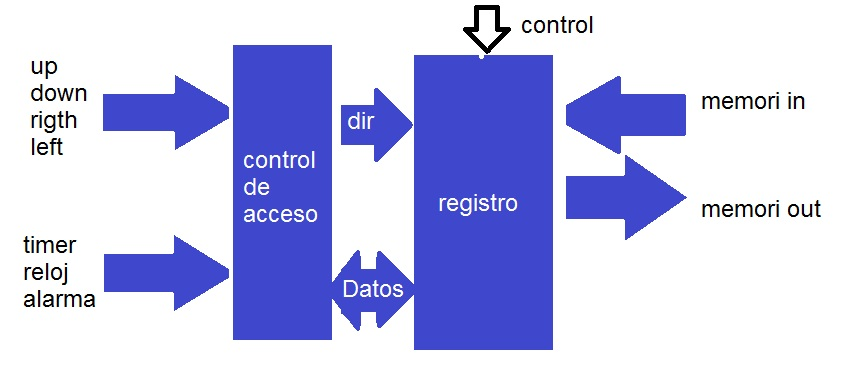
\includegraphics[height=7cm, width=16cm]{img/nivel2_contusr.jpg}
  \caption[1erNivel]{Diagrama de segundo nivel del Teclado.}
  \label{fig:SegundoNivelControlusr}
\end{figure}

\subsection{Controlador del RTC}
Para la implementación de esta interfaz que va a permitir la comunicación entre la FPGA y el RTC, se desarrolló 7 bloques principales divididos en una jerarquía de 3 niveles, se puede ver en la figura \ref{fig:Jrtc}. Existen 3 bloques principales uno de inicializacion, un while true, que permite la lectura continua de los datos de la rtc, y una de programación que permite actualizar los cambios del control de usuario.\\ [2ex]
 Ademas existen 2 bloques que permiten un bloque que permite leer y escribir datos, esta activa un control que esta basado en los tiempos de la figura \ref{fig:DTE} y la figura \ref{fig:DTL}, como se puede notar existen muchas similitudes entre ambos ciclos, para esto llamaremos a esta diferencia "ciclo" de esta manera podemos armar el cuadro de figura \ref{fig:CTS}\\[2ex]
 Este diagrama muestra los cambios que deben ocurrir según los tiempos del timer dentro del modulo, al llegar el tiempo final saca una bandera indicando el final.\\ [2ex]
\begin{figure}[htbp]
  \centering
    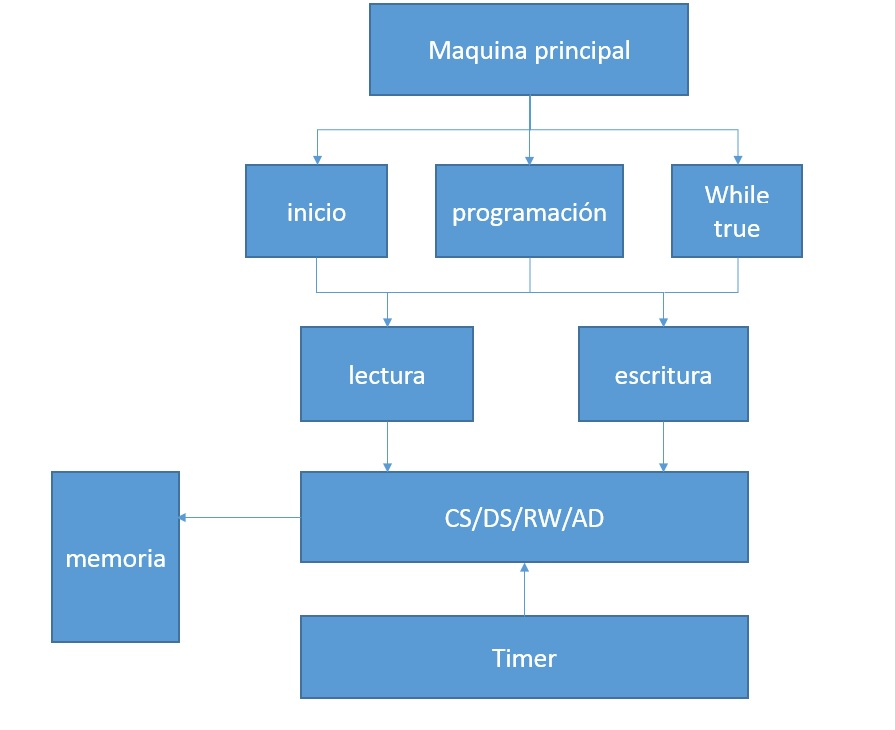
\includegraphics[height=9cm, width=16cm]{img/JerarquiaRTC.jpg}
  \caption[3erNivel]{jerarquía de la RTC.}
  \label{fig:Jrtc}
\end{figure}
\begin{figure}[htbp]
	\centering
	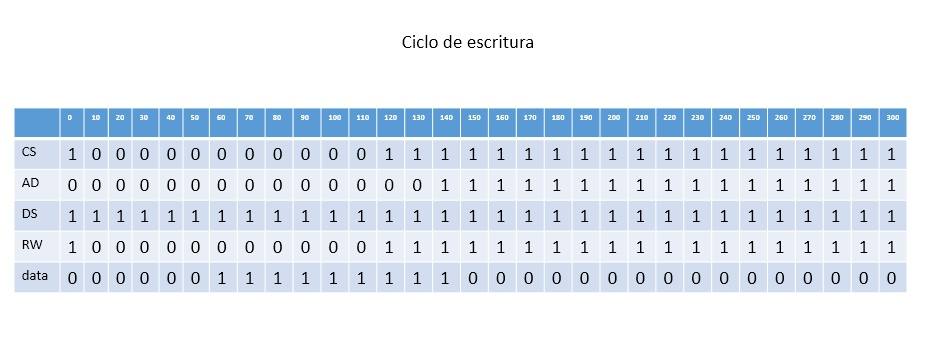
\includegraphics[height=9cm, width=16cm]{img/diagramatiempoescritura.jpg}
	\caption[3erNivel]{Diagrama de tiempos completo del ciclo de escritura.}
	\label{fig:DTE}
\end{figure}
\begin{figure}[htbp]
	\centering
	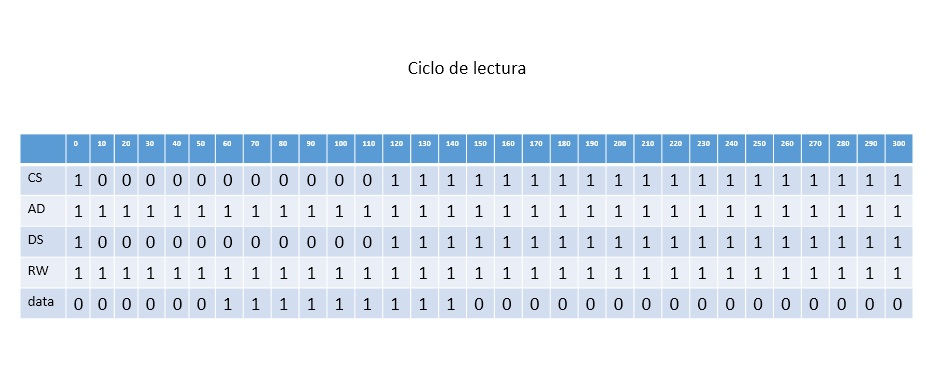
\includegraphics[height=9cm, width=16cm]{img/diagramatiempolectura.jpg}
	\caption[3erNivel]{Diagrama de tiempos completo del ciclo de lectura.}
	\label{fig:DTL}
\end{figure}
\begin{figure}[htbp]
	\centering
	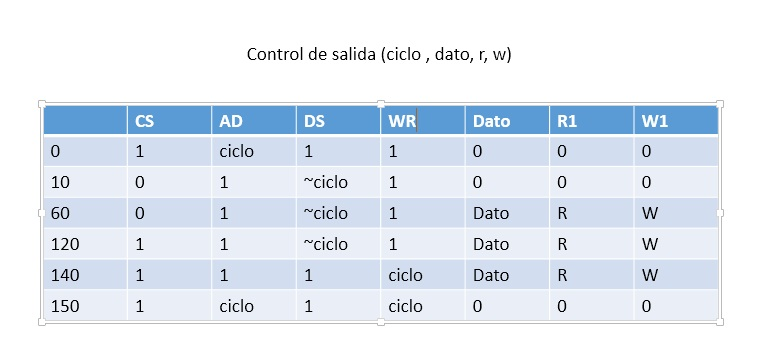
\includegraphics[height=9cm, width=16cm]{img/cuadrotiemposalida.jpg}
	\caption[3erNivel]{cuadro de tiempos del control de salida.}
	\label{fig:CTS}
\end{figure}
\subsubsection{nivel 1 control RTC}
Para este nivel se requiere la entrada y salida de datos al registro de memoria de coneccion y tiene las salidas necesarias para controlar la RTC, esto se nota en la figura \ref{fig:nivel1RTC}.\\[2ex]
\begin{figure}[htbp]
	\centering
	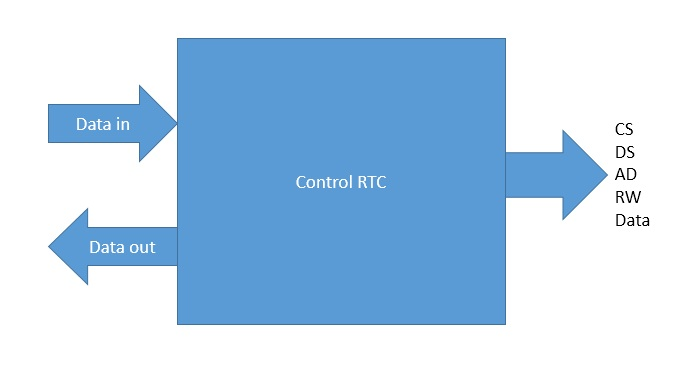
\includegraphics[height=9cm, width=16cm]{img/nivel1_RTC.jpg}
	\caption[3erNivel]{nivel 1 del RTC}
	\label{fig:nivel1RTC}
\end{figure}
\subsubsection{nivel 2 RTC}
Como se menciono antes existen 6 maquina de estados agrupados en 3 jerarquías.\\[2ex]
La primera maquina de estados es la de inicializacion, esta tiene un bit de entrada para su inicializacion. Ademas posee salidas de datos y dirección  y bits W y R, que siempre están en cero y se conectan a las maquinas de lectura y escritura respectivamente, esto responde al flujo de la figura \ref{fig:FMEI}.\\[ex]
La maquina encargada del proceso while true responde al flujo de la figura, esta tiene un bit para la iniciación de la maquina y un bit que indica que finalizo el proceso, de igual manera un bit que indica que la maquina de estados siguiente termino su proceso para que esta salte entre estados y igual que la maquina pasada tiene las señales W y R y la salida de datos y dirección.\\[2ex]
Siguiendo la jerarquía, existen 2 maquinas, escritura y lectura, estas respetan los flujos de la figura \ref{fig:FML} y \ref{fig:FME}, estas tienen las entradas de datos y dirección y la señal r y w respectivamente y tiene solo una salida de datos y r y w de esta manera las maquina controla que dato sale, si la direccion y o el dato, ademas tiene el bit de ciclo que determina si esta en el ciclo de escritura o lectura, como se nota en los flujos, el bit de ciclo no depende de la maquina, sino de la parte del programa donde esta se encuentre.\\[2ex]
Por ultimo el control de salida responde al cuadro de la figura \ref{fig:CTS} a este le entra, el bit de activación que sale de la maquina de escritura o lectura, y entran los datos del ciclo y dato que salen dependiendo del tiempo; internamente este tiene un timer, con el fin de llevar el tiempo desde la activación, y dependiendo del tiempo que transcurre genera los cambios de la figura \ref{fig:CTS}. \\[2ex]
\begin{figure}[htbp]
	\centering
	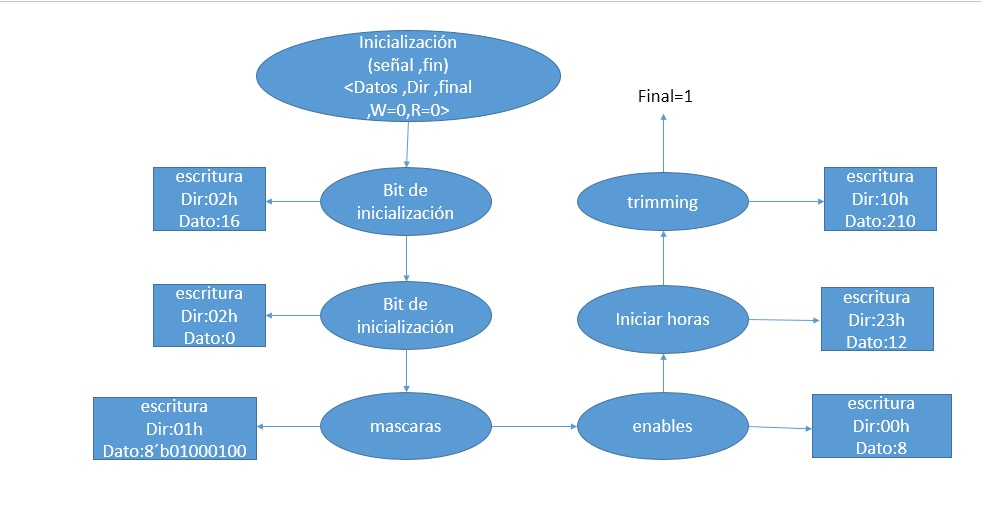
\includegraphics[height=9cm, width=16cm]{img/FlujoInit.jpg}
	\caption[3erNivel]{flujo de datos de la maquina de estados de inicializacion}
	\label{fig:FMEI}
\end{figure}
\begin{figure}[htbp]
	\centering
	\includegraphics[height=9cm, width=16cm]{img/FlujoLec.jpg}
	\caption[3erNivel]{flujo de datos de la maquina de lectura}
	\label{fig:FML}
\end{figure}
\begin{figure}[htbp]
	\centering
	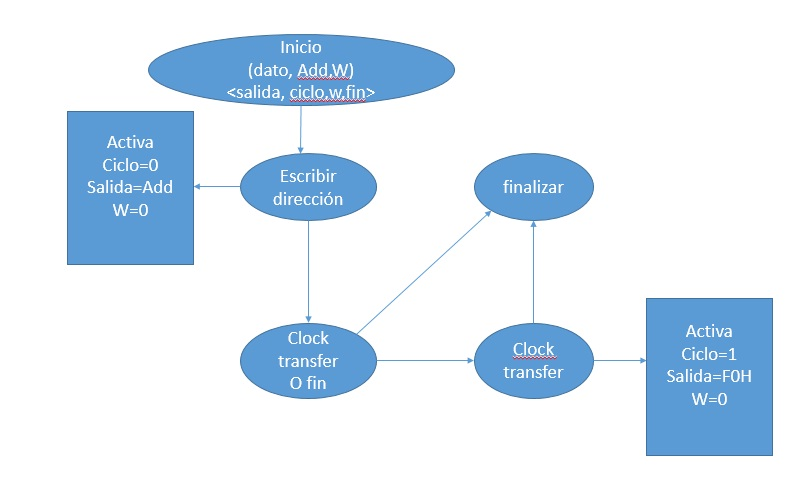
\includegraphics[height=9cm, width=16cm]{img/FlujoEsc.jpg}
	\caption[3erNivel]{flujo de datos de la maquina de Escritura}
	\label{fig:FME}
\end{figure}
\subsection{ROM de Instrucciones}


\section{Datos y resultados}
\subsection{Simulaciones}


\section{Análisis de datos y resultados}


\section{Hoja de datos de unidades desarrolladas}


\section{Conclusiones y recomendaciones}
\subsection{Conclusiones}


\subsection{Recomendaciones}


\end{document}